\documentclass[xcolor=svgnames,aspectratio=169]{beamer} 
\usetheme{metropolis}
\usefonttheme{professionalfonts}
\setbeamertemplate{theorems}[numbered]
\usepackage{luatexja}
\usepackage{luatexja-fontspec}
\usepackage{newtxtext}                     
\usepackage{amsthm} 
\usepackage{graphicx}
\usepackage{xcolor}
\usepackage{tcolorbox}
\usepackage{tikz}
\everymath{\displaystyle}
\usepackage{bm}
\usepackage{bbm}
\usepackage{lmodern}
\newcommand{\indep}{\mathop{\perp\!\!\!\!\perp}}
\newcommand{\R}{\mathbb{R}} 
\newcommand{\N}{\mathbb{N}} 
\newcommand{\Z}{\mathbb{Z}} 
\newcommand{\Q}{\mathbb{Q}} 
\newcommand{\C}{\mathbb{C}}
\newcommand{\E}{\mathbb{E}}
\newcommand{\cov}{\text{Cov}}
\newcommand{\var}{\text{Var}}

\begin{document} 

\title{Fisher-Schultz Lecture: Generic machine learning inference on heterogeneous treatment effects in randomized experiments, with an application to immunization in India \\ \small{Victor Chernozhukov et al. (2025), Econometrica (forthcoming).}}
\author{Naoki Eguchi}          
\institute{Faculty of Medicine, Kyoto University} 
\date{2025.7.9 ミクロ計量経済学}

\begin{frame}                  
    \titlepage                     
\end{frame}

\section{Introduction}

\begin{frame}{Motivation}
    \begin{itemize}
        \item When conducting RCT (Randomized Controlled Trails), reseachers and policy makers are often curious about not only ATE but also HTE (Heterogeneous Treatment Effects).
        \item In such cases, ML methods are good for estimating
    \end{itemize}
\end{frame}

\begin{frame}{Proposed estimator}
    \begin{itemize}
        \item 
    \end{itemize}
\end{frame}

\section{Main identification results and estimation strategies}

\begin{frame}{BLP (Best Linear Predictor)}
    \begin{itemize}
        \item Firstly, we obtain the estimator $S(Z)$ for CATE $s_0(Z)$ by some ML method using the auxilirary samples $\mathcal{A} $.
        \item BLP is defined as the projection of $s_0(Z)$ on the linear span of $1$ and $S(Z)$ in $L^2(P)$.
        \[
        \text{BLP}[s_0(Z)|S(Z)]=\arg\min_{f(Z)\in \text{Span}(1,S(Z))}\E[(s_0(Z)-f(Z))^2]
        \]
        \begin{itemize}
            \item This equals to the solution of $\arg\min_{b_1,b_2}\E[(s_0(Z)-b_1-b_2 S(Z))^2]$. \\
            → $\beta_1=\E[s_0(Z)], \beta_2=\frac{\cov(s_0(Z),S(Z))}{\var(S(Z))}$
        \end{itemize}

    \end{itemize}
\end{frame}

\begin{frame}{First strategy : Weighted Residual BLP}
    \begin{itemize}
        \item Consider the regresson model with the moment condition as follows.
        \begin{align*}
            Y=\alpha'X_1&+\beta_1(D-p(Z))+\beta_2(D-p(Z))(S(Z)-\E[S(Z)])+\epsilon, \E[w(Z)\epsilon X]=0 \\
            &\text{where} \  w(Z)=\frac{1}{p(Z)(1-p(Z))}, X=(X_1,X_2), \\ 
            &X_1=(1,B(Z)),X_2=(D-p(Z),(D-p(Z)(S(Z)-\E[S(Z)]))).
        \end{align*}
        \begin{tcolorbox}[colframe=Cyan,title=Theorem 1]
        \begin{itemize}
            \item Consider $z\mapsto S(z)$ and $z\mapsto B(z)$ as fixed maps. (known function)
            \item Assume that $Y$ and $X$ have finite second moments, $\E[XX']$ is full rank, and $\var(S(Z))>0$.
            \item Then, $(\beta_1, \beta_2)'=\arg\min_{b_1,b_2}\E[(s_0(Z)-b_1-b_2 S(Z))^2]$ (Identified)
        \end{itemize}
    \end{tcolorbox}
    \end{itemize}
\end{frame}

\begin{frame}{Second strategy : Horvitz-Thompson BLP}
    \begin{itemize}
        \begin{tcolorbox}[colframe=Cyan,title=Theorem 2]
        \begin{itemize}
            \item Consider $z\mapsto S(z)$ and $z\mapsto B(z)$ as fixed maps. (known function)
            \item Assume that $Y$ has finite second moments, $\E[\tilde{X}\tilde{X}']$ is finite and full rank, and $\var(S(Z))>0$.
            \item Then, $(\beta_1, \beta_2)'=\arg\min_{b_1,b_2}\E[(s_0(Z)-b_1-b_2 S(Z))^2]$ (Identified)
        \end{itemize}
    \end{tcolorbox}
    \end{itemize}
\end{frame}

\begin{frame}{GATES (sorted Group Average Treatment Effects)}
    \begin{itemize}
        \item Firstly, we build the groups by the estimated value $S(Z)$ of $s_0(Z)$.
        \[
        G_k=\{S(Z)\in I_k\}, k=1,...,K, I_k=[l_{k-1},l_k) : \text{disjoint}
        \]
        \item The estimand "GATES" is defined as $\E[s_0(Z)|G_k]$ for $k=1,...,K$.
        
    \end{itemize}
\end{frame}

\begin{frame}{Two strategies : Weihgted Residual and Horvitz-Thompson GATES}
    \begin{itemize}
        \item Consider the regression model with the moment condition as follows.
        \begin{align*}
            Y=\alpha'X_1&+\sum_{k=1}^{K}\gamma_k(D-p(Z))\mathbf{1}_{G_k}+\nu, \E[w(Z)\nu W]=0 \\
            &\text{where} W=(X_1, W_2')', W_2=\{(D-p(Z))\mathbf{1}_{G_k}\}_{k=1}^K.
        \end{align*}
    \end{itemize}
\end{frame}

\begin{frame}{Identification of GATES}
    \begin{itemize}
        \begin{tcolorbox}[colframe=Cyan,title=Theorem 3]
        \begin{itemize}
            \item Consider $z\mapsto S(z)$ and $z\mapsto B(z)$ as fixed maps. (known function)
            \item Assume that $Y$ has finite second moments and  both $\E[WW']$ and $\E[\tilde{W}\tilde{W}']$ are finite and full rank.
            \item Then, $\gamma=\{\gamma_k\}_{k=1}^K$ defined in two different ways are equivalent and identified.
            \[
            \gamma_k=\E[s_0(Z)|G_k]
            \]
        \end{itemize}
    \end{tcolorbox}
    \end{itemize}
\end{frame}

\begin{frame}{CLAN (Classification Analysis)}
    \begin{itemize}
        \item When BLP and GATES reveal substantial heterogeneity, it is interesting to know \alert{the properties of the subpopulations} that are most and least affected.
        \begin{itemize}
            \item We focus on the "least affected group" $G_1$ and "most affected group" $G_K$.
        \end{itemize}
        \item Let $g(Y,Z)$ be a vector of characteristics of an observational unit. The estimands are 
        \[
        \delta_1=\E[g(Y,Z)|G_1]\quad \text{and}\quad\delta_K=\E[g(Y,Z)|G_K]
        \]
        \item These parameters are identified with no assumption because they are just average of observed variables.
        \item We compare $\delta_1$ and $\delta_K$ to detect (single out) the covariates which causes the heterogeneity.
        \begin{itemize}
            \item We can extend the comparison of not only averages but also variances or distributions.
        \end{itemize}
    \end{itemize}
\end{frame}

\section{"Variational" estimation and inference methods}

\begin{frame}{Uncertainty}
    \begin{itemize}
        \item Let $\theta$ denote a generic target parameter such as BLP $\beta_2$ or GATE $\gamma_k$.
        \item There are two principal sources of sampling uncertainty.
        \begin{itemize}
            \item \alert{Estimation uncertainty} regarding the parameter $\theta$, conditional on the data subpopulations
            \item Uncertainty or "variation" \alert{induced by the data splitting}
        \end{itemize}
        \item Actually, estimation uncertainty is a standard topic, so, as usual, we can solve this problem by the \alert{Gaussian approximation} to construct a confidence interval.
        \item On the other hands, data-splitting uncertainty is a novel topic, which is solved by taking a \alert{median} of any estimators in permuated splitting. 
    \end{itemize}
\end{frame}

\begin{frame}{Estimation uncertainty in single split}
    \begin{itemize}
        \item Consider a sample split $\{(a,m)\}$ of $\{1,...,N\}$ with $|a|=N-n, |m|=n$.
        \item All estimators $\theta_a$ satisfies the sufficient conditions for being approxmately Gaussian, conditionally on $Data_a$.
        \[
        P(\frac{\hat{\theta_a}-\theta_a}{\hat{\sigma_a}}<z|Data_a) \to \Phi(z) \ \text{for} \ z\in\R, \ \text{as} \ N \ \text{and} \ n\to\infty
        \]
        \item 
    \end{itemize}
\end{frame}

\begin{frame}{Splitting uncertainty in multiple splits}
    \begin{itemize}
        \item 
    \end{itemize}
\end{frame}

\section{Causal machines that learn CATE better}

\begin{frame}{Athey and Imbens (2016) : Resursive partitioning tree method}
    \begin{itemize}
        \item 
    \end{itemize}
\end{frame}

\begin{frame}{Nie and Wager (2021) : R-learner}
    \begin{itemize}
        \item 
    \end{itemize}
\end{frame}

\begin{frame}{Causal learners for Stage 1}
    \begin{itemize}
        \item In Stage 1, using the auxilirary sample $A$, we estimate 
        \begin{itemize}
            \item BCA (Baseline Conditional Average) : $b_0(Z)=\E[Y(0)|Z]$
            \item CATE (Conditional Average Treatment Effect) : $s_0(Z)=\E[Y(1)-Y(0)|Z]$
        \end{itemize}
        → solve \alert{either} of Weighted Residual (WR) learner or Horvitz-Thompson (HT) learner.
        \begin{align*}
            &(B,S)\in \arg\min_{b\in\mathcal{B} , s\in\mathcal{S} }\sum_{i\in A} \footnote{以後は簡単のため, $w(Z)=\frac{1}{p(Z)(1-p(Z))}$と表記する.}\frac{1}{p(Z_i)(1-p(Z_i))}\{Y_i-b(Z_i)-(D_i-p(Z_i))s(Z_i)\}^2 \\
            &(B,S)\in \arg\min_{b\in\mathcal{B} , s\in\mathcal{S} }\sum_{i\in A} \{\footnote{以後は簡単のため, $H=\frac{D-p(Z)}{p(Z)(1-p(Z))}$と表記する.}\frac{D_i-p(Z_i)}{p(Z_i)(1-p(Z_i))}(Y_i-b(Z_i))-s(Z_i)\}^2 
        \end{align*}
        \begin{center}
            where $\mathcal{B}$ and $\mathcal{S}$ are functional parameter spaces
        \end{center}
    \end{itemize}
\end{frame}

\begin{frame}{Oracle properties of the population objective functions}
    \begin{itemize}
        \begin{tcolorbox}[colframe=Cyan,title=Theorem 4]
        \begin{itemize}
            \item Suppose $Y, b(Z), s(Z), w(Z) \in L^2$ (2乗可積分).
            \item Then, the expectation of the loss functions can be decomposed 
            \begin{align*}
                &\E[w(Z)\{Y-b(Z)-(D-p(Z))s(Z)\}^2]=\E[(s_0(Z)-s(Z))^2]+C_{ib} \\
                &\E[(H(Y-b(Z)-s(Z)))^2]=\E[(s_0(Z)-s(Z))^2]+C_{2b}
            \end{align*}
            where $C_{1b}=\E[w(Z)(\tilde{b}_0(Z)-b(Z))^2]+C_1, C_{1b}=\E[w(Z)(\bar{b}_0(Z)-b(Z))^2]+C_2$
        \end{itemize}
    \end{tcolorbox}
    \item This theorem shows that the minimizers provide the best approxmation for $s_0(Z)$ in the sense of mean-squared error in the class $\mathcal{S} $.
    \item Moreover, this occurs even though we do not know $s_0(Z)$. (oracle!)
    \end{itemize}
\end{frame}

\begin{frame}
    \begin{figure}
            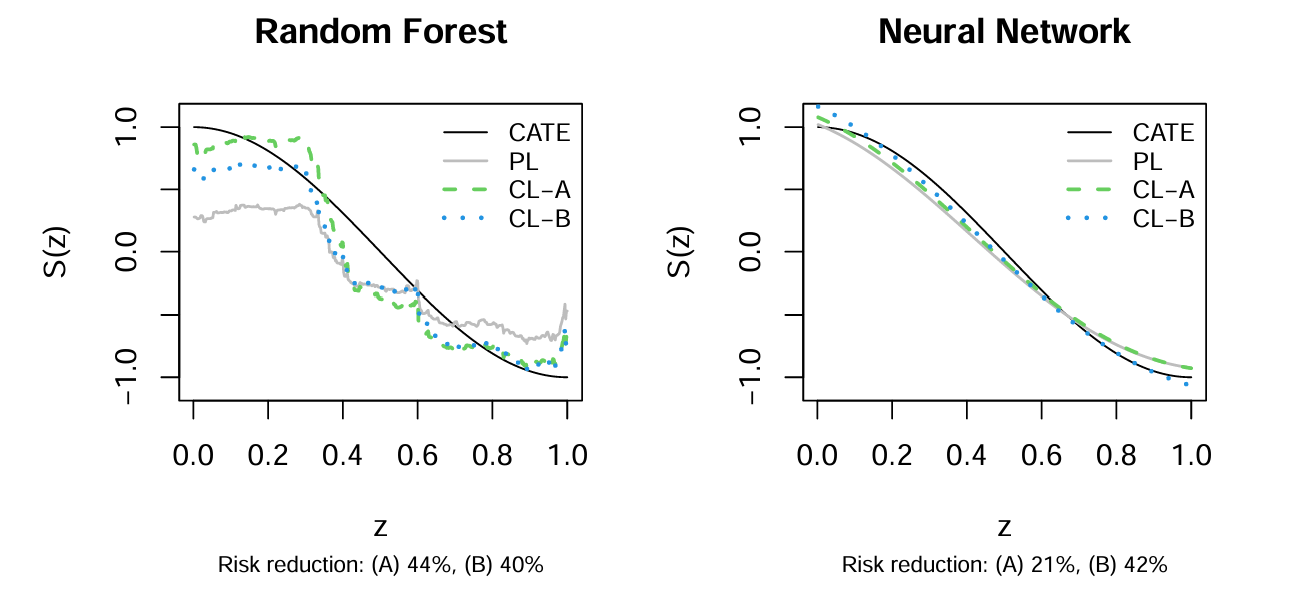
\includegraphics[width=1.5\textwidth, height=0.4\textheight, keepaspectratio]{PLvsCL(RF,NN).png}
        \end{figure}
    \begin{itemize}
        \item 
    \end{itemize}
\end{frame}

\begin{frame}
    \begin{figure}
            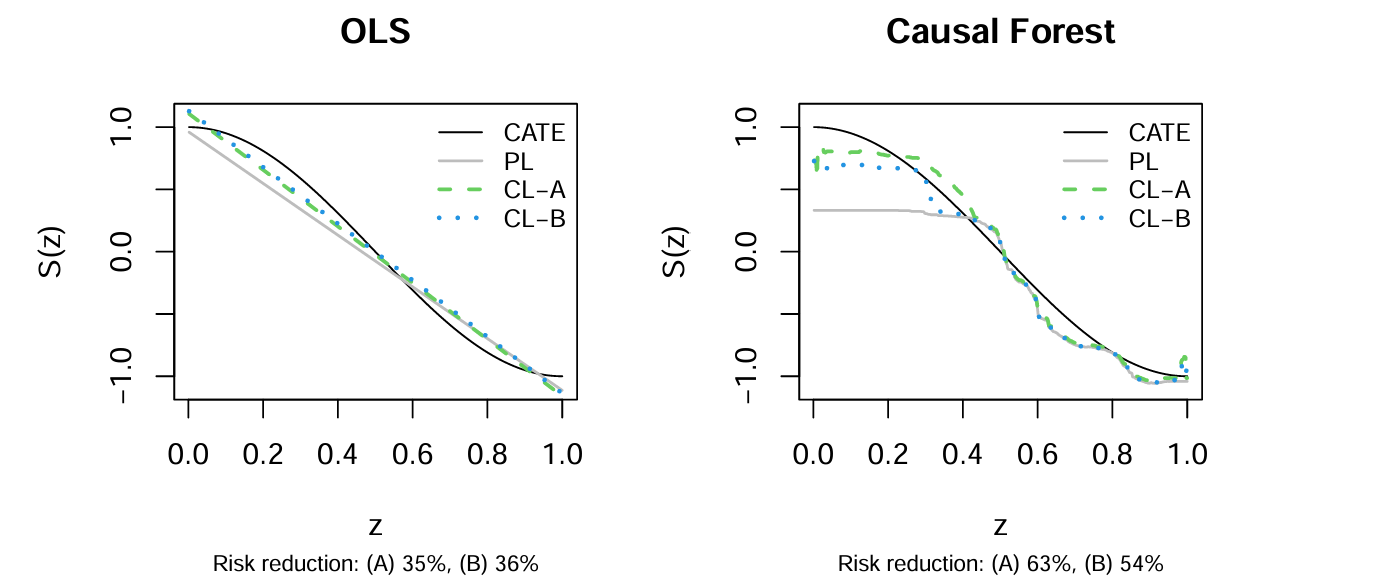
\includegraphics[width=1.5\textwidth, height=0.4\textheight, keepaspectratio]{PLvsCL(OLS,CF).png}
        \end{figure}
\end{frame}

\section{Implementation Details}

\begin{frame}{Inference algorithm 1}
    \begin{enumerate}
        \item 
    \end{enumerate}
\end{frame}

\begin{frame}{Inference algorithm 2}
    \begin{enumerate}
        \item 
    \end{enumerate}
\end{frame}

\section{Final marks}

\section{References}

\begin{frame}{References}
    \begin{itemize}
        \item Victor Chernozhukov, Mert Demirer, Esther Duflo, and Iván Fernández-Val (2025), \textit{Fisher-Schultz Lecture: Generic machine learning inference on heterogeneous treatment effects in randomized experiments, with an application to immunization in India}, Econometrica (forthcoming).
        \item Xinkun Nie, Stefan Wager (2021), \textit{Quasi-Oracle Estimation of Heterogeneous Treatment Effects}, Biometrika.
        \item Susan Athey, Guido Imbens (2016), \textit{Recursive partitioning for heterogeneous causal effects}, Proceedings of the National Academy of Sciences. 
        \item Kosuke Imai and Michael Lingzhi Li (2025), \textit{Statistical Inference for Heterogeneous Treatment Effects Discovered by Generic Machine Learning in Randomized Experiments}, Journal of Business and Economic Statistics. 
        \item 金本拓 (2024), 因果推論ー基礎からの機械学習・時系列解析・因果探索を用いた意思決定のアプローチー, オーム社. (主に5章)
    \end{itemize}
\end{frame}

\end{document}